\chapter{Transport layer}
\lecture{4}{29/10}

Transport services and protocols provide \emph{logical communication} between application processes running on different hosts. Transport protocols run in the end system. There are two sides to the network layer:
\begin{enumerate}
    \item \emph{send side}, this breaks up application messages into \emph{segments} and passes it to the network layer; and
    \item \emph{receive side}, this reassembkes the segments into messages then passes it to the application layer.
\end{enumerate}

There are more than one transport protocol available to apps (TCP and UDP). 

When we compare the network layer and the transport layer, we see that the network layer provies logical communication between \emph{hosts} while the transport layer provides logical communication between \emph{processes}. The transport layer relies on the network layer services. 

Recall TCP and UDP, these extend the IP delivery service between hosts to deliver a service between processes.

\section{Multiplexing and demultiplexing}

\begin{definition}[Multiplexing]
    \textbf{Multiplexing} (or \textbf{muxing}) is a method by which multiple signals are combined over a single medium.
\end{definition}

The aim of multiplexing is to share a single scarce resource, such as a link between two hosts. When multiplexing, routers typically add a \emph{transport header} that specifies the source and destination port number. Each datagram already has the source and destination IP addresses, so when a router receives a datagram it can decided where to send them. Figure \ref{fig:segment-example} shows the format of a TCP/UDP segment.

\begin{figure}
    \centering
    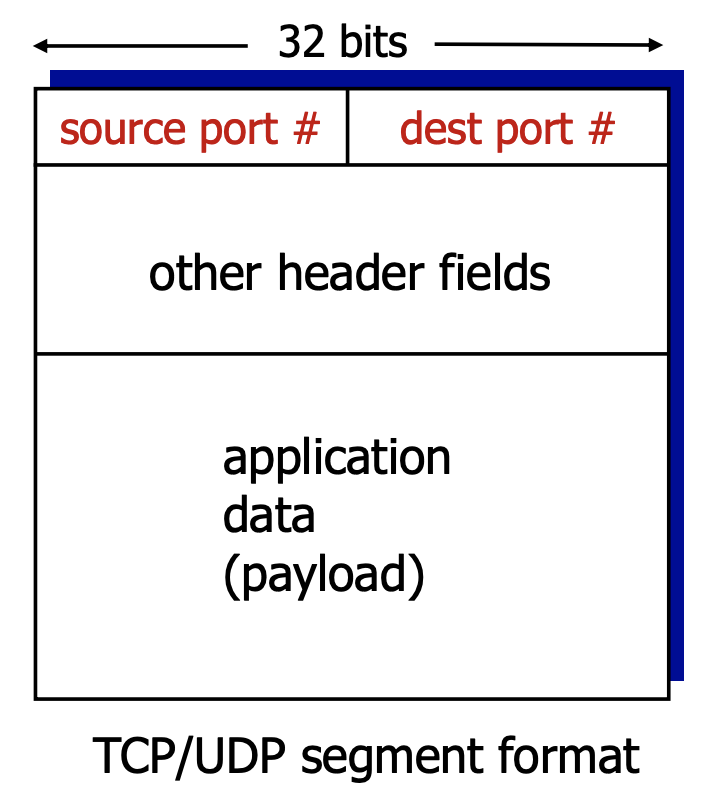
\includegraphics[width=0.6\linewidth]{images/segment-example.png}
    \caption{An example TCP/UDP segment formal.}
    \label{fig:segment-example}
\end{figure}

\begin{definition}[Demultiplexing]
    \textbf{Demultiplexing} (or \textbf{demuxing}) is the process of using heading information to deliever the received segments to the correct socket.
\end{definition}

All sockets have a host-local port number which is typically assigned automatically. 

When a host receives a UDP segment, it checks the destination port number in the segment then directs the UDP segment to the socket with that port number. 
If two UDP segments have different source IP addresses and or source port numbers but the same destination IP and port number then they will be directed to the same process via the same socket at the destination.

TCP sockets are identified by a $4$-tuple containing the source IP address, the source port number, the destination IP address, and the destination port number. Demuxers receive all four of these valuesss and uses it to direct the segment to the appropriate socket. Servers may host many simulateneous TCP sockets; however, two arriving TCP segments with different source IP addresses and port numbers will be directed to two different sockets.

\section{Principles of reliable data transfer}

If we are sending data along a unreliable channel, the characteristics of this channel will determine the complexity of a reliable data transfer protocol. 
Data enters the transfer layer via a \texttt{rdt\_send()} call, this passes the data to the upper layer. 
Then \texttt{udt\_send()}, which is called by the protocol, transfers the packet over to the unreliable channel. 
\texttt{rdt\_rcv()} is called when the packet is received and must go through the receive side of the transport layer. 
Once the message has been reconstructed \texttt{deliver\_data()} is called to deliver the data to the application layer.
